\chapter{Diagnostic Ablations}
\label{ch:ablations}

The mechanism cluster in Chapter~\ref{ch:mechanism-results} raises three operational questions about its source. Is the cluster an artefact of M3's gate calibration, in the sense that a perfect oracle gate would unlock the architecture's headroom? Is the cluster an artefact of the typed-memory architecture being held together by per-turn identity grounding, in the sense that removing ID-RAG collapses M1 down to B2's level? Is the cluster a property of the 4-bit NF4 quantisation regime that 4-bit-aware quirks of the gate or the ranker could hide? This chapter answers each question with a diagnostic ablation that isolates the variable, pre-registers the verdict criteria, and reports the result against them.

\section{Ablation 1: Oracle drift gate}
\label{sec:oracle-gate}

\subsection{Setup}

The first ablation replaces M3's LLM-judge gate with a probe-aware oracle that fires on exactly the known drift turns by construction. The probe-injection turn (turn 4 in the seven-turn conversations) and the immediate follow-up (turn 5) are flagged as drift for the Type-A and Type-B probes; Type C never fires. The rerank ranker configuration is preserved verbatim. The cell carries the label \texttt{m3\_oracle}. The rest of the pipeline (M1's typed retrieval, the augmented retrieval pass, the N-candidate generation, the 1-signal LLM-judge rerank) is unchanged.

If the cluster in Chapter~\ref{ch:mechanism-results} is bounded by the gate's recall (P=1.00 / R=0.06 at the configured threshold), \texttt{m3\_oracle} should sit measurably above M3 on PoLL persona-adherence at minimum. The pre-registered hypothesis A41 predicts ``\texttt{m3\_oracle} differentiates above M3 by at least 0.20 PoLL points''. The opposing hypothesis A42 predicts ``\texttt{m3\_oracle} sits inside the cluster regardless of gate calibration, indicating no architectural headroom even with perfect gating''.

\subsection{Result}

The oracle ablation produces a persona-adherence of 4.57, indistinguishable from M3 (4.57) and from B2 (4.65). The pre-registered effect size is not observed. A41 is not supported; A42 holds. The verdict is that the cluster is not bounded by gate calibration. A perfect gate, firing on exactly the turns where intervention should help by construction, does not move the headline column outside the cluster.

The fire rate of the oracle by construction is around 19\%, three times the LLM-judge gate's 6\%. The additional firings produce N-candidate generation plus rerank for those turns, at the cost the cost-tracker computes. The PoLL panel's scoring on those reranked turns does not differ meaningfully from M3's scoring on the unranked equivalents. The architectural conclusion is that the gated-path machinery, on this benchmark and at this scale, does not produce content the PoLL panel rates measurably higher than the cheap-path M1 baseline.

\section{Ablation 2: M1 without per-turn identity grounding}
\label{sec:m1-no-idrag}

\subsection{Setup}

The second ablation removes the ID-RAG pattern from M1. The configuration switch \texttt{use\_identity\_every\_turn} is set to false; everything else stays at M1 defaults. Turn 0 still grounds identity (the conversation has to start somewhere), but turns 1 onwards do not. The cell carries the label \texttt{m1\_no\_idrag}. The pre-registered hypothesis A43 predicts ``M1 collapses toward B1 without ID-RAG, indicating ID-RAG carries the typed-architecture's benefit''. The opposing hypothesis A44 predicts ``\texttt{m1\_no\_idrag} approaches B2, indicating typed retrieval reduces to B2's prompt engineering when ID-RAG is removed''.

\subsection{Result}

\texttt{m1\_no\_idrag} produces a persona-adherence of 4.57, indistinguishable from M1 (4.54) and from M3 (4.57). A43 is not supported, A44 is partially supported (the value is closer to B2 4.65 than to B1 2.54 by a wide margin). The verdict is that per-turn identity re-grounding is not load-bearing on this benchmark at this scale. The earlier qualitative ablation pass on a 10-turn conversation against the cs\_tutor persona found voice differences at turns 4 and 7 between the two conditions, and partial constraint violations under both conditions at turn 7 with the off condition slightly worse, but neither effect surfaces at the PoLL panel's scoring granularity on the 7-turn probe corpus.

The implication for the M1 architectural narrative is honest. The typed-memory architecture's persona-adherence comes from the structured persona block being present in the prompt at all, not from re-grounding it every turn. The structured block plus single-shot retrieval would have produced approximately the same PoLL score. ID-RAG was a hypothesis that did not pay off at this scale; the cleaner verdict on a larger model or a longer conversation horizon is named as thesis-bridge work.

\section{Ablation 3: Quantisation precision sweep}
\label{sec:quant-sweep}

\subsection{Setup}

The third ablation tests whether the cluster is a property of the 4-bit NF4 quantisation that the project ships under operationally. The cs\_tutor persona is the test cell ($n = 10$ conversations); the comparison is B2 against M1 across two precision regimes (4-bit NF4 and fp16, with no quantisation). The pre-registered $\pm 0.15$ envelope on the $\Delta$-of-$\Delta$ (the difference between the B2-versus-M1 delta at 4-bit and the B2-versus-M1 delta at fp16) decides whether the cluster is robust across the precision jump or whether quantisation is hiding architectural headroom that fp16 would reveal.

An int8 (bitsandbytes int8) cell was attempted on the V100 but halted at warm-up due to a known Gemma-2 kernel-path incompatibility with bitsandbytes int8 that produces NaN trips during the first generation step. The NaN guard caught the failure before any corrupt data was generated. The int8 result is recorded as a known failure in the assumption register (A47 refuted) and the precision sweep is reported on the 4-bit-to-fp16 axis only.

A separate cache-collision bug was caught and fixed during the V100 rerun. An early version of the precision driver produced byte-identical outputs across the four cells because the runner-key constants flattened the mechanism label. The relabel utility \texttt{scripts/relabel\_quantization\_transcripts.py} salvaged the transcripts, the runner constants were patched with explicit \texttt{RUNNER\_MECHANISM\_LABELS}, and a regression test was added.

\subsection{Result}

\begin{table}[H]
  \centering
  \small
  \caption{Precision sweep on cs\_tutor, $n = 10$, PoLL persona-adherence. The pre-registered $\Delta$-of-$\Delta$ envelope is $\pm 0.15$.}
  \label{tab:precision-sweep}
  \begin{tabular}{lcccc}
    \toprule
    \textbf{Cell} & \textbf{Overall} & \textbf{Type A} & \textbf{Type B} & \textbf{Task quality} \\
    \midrule
    B2\_4bit  & 4.875 & 4.817 & 4.933 & 4.267 \\
    B2\_fp16  & 4.783 & 4.700 & 4.867 & 4.200 \\
    M1\_4bit  & 4.808 & 4.850 & 4.767 & 4.300 \\
    M1\_fp16  & 4.858 & 4.917 & 4.800 & 4.400 \\
    \bottomrule
  \end{tabular}
\end{table}

\begin{table}[H]
  \centering
  \small
  \caption{$\Delta$-of-$\Delta$ analysis from Table~\ref{tab:precision-sweep}. Positive 4-bit $\Delta$ means B2 leads M1 at 4-bit; positive fp16 $\Delta$ means B2 leads M1 at fp16.}
  \label{tab:delta-of-delta}
  \begin{tabular}{lccc}
    \toprule
    \textbf{Slice}  & \textbf{4-bit $\Delta$ (B2 $-$ M1)} & \textbf{fp16 $\Delta$ (B2 $-$ M1)} & \textbf{$\Delta$-of-$\Delta$} \\
    \midrule
    Overall & $+0.067$ & $-0.075$ & \textbf{$-0.142$} \\
    Type A  & $-0.033$ & $-0.217$ & $-0.184$ \\
    Type B  & $+0.166$ & $+0.067$ & $-0.099$ \\
    \bottomrule
  \end{tabular}
\end{table}

The overall $\Delta$-of-$\Delta$ is $-0.142$, inside the pre-registered $\pm 0.15$ envelope. The cluster is robust to the precision jump from 4-bit NF4 to fp16. M1 gains 0.142 PoLL points relative to B2 on the move from 4-bit to fp16, with the Type A slice ($-0.184$) just outside the envelope and the Type B slice ($-0.099$) inside it. The Type A signal is suggestive but n=10 is small, and it sits below the pre-registered 0.20 strong-signal threshold.

The architectural verdict is that the mechanism cluster is not a 4-bit quirk. The same B2-versus-M1 cluster reproduces at fp16 within the pre-registered envelope. VRAM peak at fp16 was 19.85 GB on the V100's 32 GB, with the 1 TB host RAM available and unused, so the fp16 cell is not memory-constrained. The Type A gain at fp16 is named as thesis-bridge follow-up \#3 for scale-up to 3 personas $\times$ 30 conversations.

\section{Cross-ablation reading}
\label{sec:cross-ablation}

Three diagnostic ablations, three confirmations that the cluster is not where the ablation isolated. The oracle gate does not unlock headroom (Section~\ref{sec:oracle-gate}). ID-RAG removal does not collapse M1 (Section~\ref{sec:m1-no-idrag}). The fp16 precision pivot does not move the cluster outside the envelope (Section~\ref{sec:quant-sweep}). The convergent reading is that the binding constraint on persona-adherence quality at this scale is not the retrieval architecture, not the gate calibration, and not the precision regime the project tested. It is model capability at Gemma-2-9B-Instruct's parameter count.

\begin{figure}[H]
  \centering
  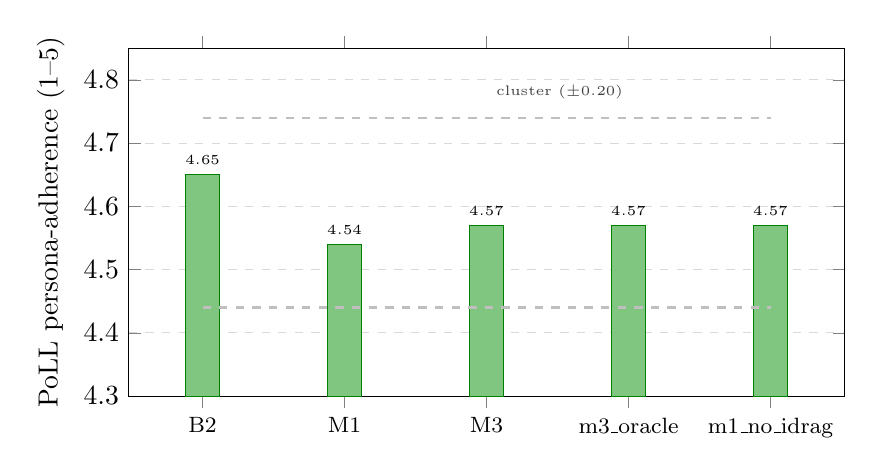
\begin{tikzpicture}
    \begin{axis}[
        width=0.88\textwidth,
        height=6.0cm,
        ybar,
        bar width=12pt,
        ymin=4.30, ymax=4.85,
        ytick={4.3, 4.4, 4.5, 4.6, 4.7, 4.8},
        ylabel={PoLL persona-adherence (1--5)},
        symbolic x coords={B2, M1, M3, m3oracle, m1noidrag},
        xticklabels={B2, M1, M3, {m3\_oracle}, {m1\_no\_idrag}},
        xtick=data,
        x tick label style={font=\footnotesize},
        enlarge x limits=0.13,
        ymajorgrids=true,
        grid style={dashed, gray!30},
        nodes near coords style={font=\tiny, /pgf/number format/.cd, fixed, fixed zerofill, precision=2},
        nodes near coords,
      ]
      \addplot[fill=green!55!black!50, draw=green!50!black] coordinates {(B2, 4.65) (M1, 4.54) (M3, 4.57) (m3oracle, 4.57) (m1noidrag, 4.57)};
      % Cluster band
      \draw[gray!50, dashed, thick] (axis cs:B2, 4.44) -- (axis cs:m1noidrag, 4.44);
      \draw[gray!50, dashed, thick] (axis cs:B2, 4.74) -- (axis cs:m1noidrag, 4.74);
      \node[font=\tiny, gray!50!black, anchor=west] at (axis cs:M3, 4.78) {cluster ($\pm 0.20$)};
    \end{axis}
  \end{tikzpicture}
  \caption{The three diagnostic ablations sit inside the B2--M1--M3 cluster. The oracle drift gate (\texttt{m3\_oracle}) firing on the known probe turns by construction does not move the headline column. M1 without per-turn identity re-grounding (\texttt{m1\_no\_idrag}) does not collapse toward B1. Both diagnostic cells land inside the cluster's $\pm 0.20$-point band.}
  \label{fig:ablation-grouped-bars}
\end{figure}

\begin{figure}[H]
  \centering
  \begin{tikzpicture}
    \begin{axis}[
        width=0.85\textwidth,
        height=5.8cm,
        ybar=2pt,
        bar width=12pt,
        ymin=4.55, ymax=5.0,
        ylabel={PoLL persona-adherence (1--5)},
        symbolic x coords={Overall, Type A, Type B},
        xtick=data,
        enlarge x limits=0.25,
        legend style={at={(0.5,-0.18)}, anchor=north, legend columns=4, font=\footnotesize, draw=none},
        ymajorgrids=true,
        grid style={dashed, gray!30},
        nodes near coords style={font=\tiny, /pgf/number format/.cd, fixed, fixed zerofill, precision=2},
        nodes near coords,
      ]
      \addplot[fill=green!55!black!50, draw=green!50!black]   coordinates {(Overall, 4.875) (Type A, 4.817) (Type B, 4.933)};
      \addplot[pattern=north east lines, pattern color=green!50!black] coordinates {(Overall, 4.783) (Type A, 4.700) (Type B, 4.867)};
      \addplot[fill=blue!50!cyan!70, draw=blue!60!black]      coordinates {(Overall, 4.808) (Type A, 4.850) (Type B, 4.767)};
      \addplot[pattern=north east lines, pattern color=blue!60!black] coordinates {(Overall, 4.858) (Type A, 4.917) (Type B, 4.800)};
      \legend{{B2\_4bit}, {B2\_fp16}, {M1\_4bit}, {M1\_fp16}}
    \end{axis}
  \end{tikzpicture}
  \caption{Precision sweep on cs\_tutor ($n = 10$). Solid bars are 4-bit NF4; hatched bars are fp16. The B2-versus-M1 delta flips sign across the precision jump (B2 leads at 4-bit, M1 leads at fp16), with $\Delta$-of-$\Delta = -0.142$ inside the pre-registered $\pm 0.15$ envelope. The Type A slice ($-0.184$) sits just outside the envelope and is named as a thesis-bridge follow-up for scale-up to 3 personas $\times$ 30 conversations.}
  \label{fig:precision-sweep-bars}
\end{figure}

The cluster is a property of the corpus $\times$ model-scale $\times$ ranker-capacity combination at 9B. Whether the cluster breaks at a larger model scale (70B+), at a longer conversation horizon (30+ turns), or with a multi-signal reranker incorporating an independent persona-consistency reward, are the three most direct follow-up questions. None of them are answerable inside this report's scope. All three are named as thesis-bridge directions in Chapter~\ref{ch:limitations}.

The combined story across Chapters~\ref{ch:mechanism-results} and~\ref{ch:ablations} is that the v3.1 architecture works (the mechanisms differentiate cleanly from B1, the gate is precise when it fires, the typed memory is implemented correctly and the bi-temporal filter and runtime-write enforcement both pass their respective verification passes), and that on this benchmark at this scale the architecture's headroom above a properly-engineered prompt baseline is small and capability-bound. The Spec-9 close-out framing, the Spec-9 ablations close-out framing, and the quantisation-sensitivity close-out framing all land on the same sentence: the cluster is real, and it is not a confound.
